\section{Hardware}

\subsection{Introducci\'on}
\label{Hintro}
Para nosotros, un robot recolector de residuos deb\'ia contar con caracter\'isticas que permitieran el sensado de un entorno f\'isico y din\'amico,
actuar seg\'un sus prop\'ositos y le proveyeran del mayor nivel de autonom\'ia energ\'etica y de interacci\'on humana posible.

Deb\'ia tener capacidades para reconocer distintos objetos en su campo de visi\'on y puder discernir entre la basura para recogerla y un
obst\'aculo para evitarlo.

Deb\'ia poder desplazarse por una terraza y tener informaci\'on de su posici\'on respecto a la base para mantener a la bater\'ia recargada y
el recipiente interno disponible para nuevos res\'iduos. Tambi\'en deber\'ia poder seguir una l\'inea para dirigirse a la base o recalibrar
su posici\'on actual.

Seg\'un las especificaciones dadas, tuvimos en cuenta varias posibles implementaciones que explicamos y analizamos en la secci\'on \ref{HposiblesDisenos}.
Detallamos los distintos dispositivos de sensado, modos de locomoci\'on y actuadores que tuvimos en cuenta, sus caracter\'isticas principales y por qu\'e
los elegimos para la construcci\'on del robot.

En las secciones \ref{Hactuadores} y \ref{Hsensores} vemos, respectivamente, los actuadores y sensores que utilizamos finalmente para el armado
f\'isico del robot.
En la secci\'on \ref{Hcomm} analizamos cuestiones con respecto a la comunicaci\'on interna entre los distintos dispositivos.
Finalmente en la secci\'on \ref{Harmado} mostramos aspectos de contrucci\'on, desde el dise\~no y armado de las placas controladoras hasta la
construcci\'on del primer prototipo del robot.

\subsection{Posibles dise\~nos e implementaci\'on}
\label{HposiblesDisenos}

Evaluamos distintos factores para la elecci\'on de cada dispositivo o m\'odulo presente en el robot. Desde la forma de sensado hasta el
tipo de ruedas, pasando por el controlador, captura de im\'agenes y m\'etodo de recolecci\'on de residuos. Estos son los factores que explicamos y
detallamos en este apartado.

\subsubsection{Sensado}

El sensado del ambiente englobaba varios puntos que deb\'iamos tener en cuenta a la hora de elegir la cantidad, forma, rango, m\'etodo y costo
de los sensores. En principio los requerimientos eran claros, necesitabamos poder detectar objetos en el ambiente, evitar obst\'aculos y realizar
mediciones internas al robot, como eran el nivel de bater\'ia, consumos y posici\'on de los motores.

La captura de im\'agenes deb\'ia ser realizada por medio de una c\'amara de video o webcam. Esta prove\'ia de la principal fuente de datos para
el proceso de reconocimiento de residuos explicado en el documento. Las distintas caracter\'isticas de la c\'amara como su resoluci\'on, refresco,
nivel de ruido, mejoras de la im\'agen y su velocidad de respuesta nos determinar\'ian la elecci\'on de la misma.

La detecci\'on de obst\'aculos implicaba otras caracter\'istcas de sensores. Principalmente de necesitabamos sensores de distancia con la apertura
necesaria para cubrir el per\'imetro del robot lo mejor posible y otorgando un rango de detecci\'on lo suficientemente olgado permitiendo una adecuada
velocidad de respuesta al controlador principal para reacci\'onar y poder evitar objetos desconocidos o marcados como obst\'aculos.

Entre los distintos tipos de sensores de distancia estaban los de ultrasonido, tel\'emetros infrarrojos y scanners l\'aser. Los sensores de distancia
por ultrasonido tienen un rango aproximado entre 2 cent\'imetros y 4 metros en la zona de detecci\'on y un \'angulo de apertura variable seg\'un la
distancia al objetivo. Tienen un \'unico inconveniente que es el tiempo de espera que se debe tener entre disparo y disparo del sensor por posibles
rebotes del pulso de sonido, lo que no lo hace adecuado para la colocaci\'on a lo largo del per\'imetro del robot. En contraparte los tel\'emetros 
infrarrojos no poseen esta limitaci\'on debido a la muy superior velocidad de la luz respecto a la del sonido. Pero el rango efectivo de detecci\'on
de objetos es de $4$ a $30$ cent\'imetros.

Debido a las caracter\'isticas de los sensores se decidi\'o combinarlos para aprovechar los beneficios de cada uno de ellos y suplir las falencias
de un tipo con otro el tipo. Un anillo de 8 tel\'emetros distribuidos de forma tal que haya una mayor resoluci\'on en la zona frontal del robot
contra la zona trasera y lateral y un \'unico sensor de distancia por ultrasonido al frente para captar objetos a mayor distancia.

El uso de un scanner l\'aser ser\'ia ideal para un an\'alisis topogr\'afico del terreno pero no es el caso y el elevado costo de los mismos los
deja fuera de escala para el proyecto.

La detecci\'on de una l\'inea en el piso la resolvimos mediante el uso de sensores opticos reflectivos apuntando hacia el piso de manera tal que
permitieran diferenciar entre distintos niveles de reflexi\'on y por ende, diferenciar una l\'inea del piso.

Las caracter\'isticas de los sensores elegidos se explican con m\'as detalles en la secci\'on \ref{Hsensores}.

\subsubsection{Locomoci\'on}

Por tratarse de un robot movil, la locomoci\'on fue un factor importante que tubvimos en cuenta. En un principio la forma en que el robot iba a desplazarse,
si iba a ser mediante ruedas, orugas o patas. En segundo t\'ermino, requer\'iamos poder determinar y asegurar la velocidad a la cual se desplazaba,
saber la cantidad y sentido del desplazamiento y conocer su consumo.

La coordinaci\'on de las patas y el equilibrio del cuerpo implicaba una complejidad que escapaba el alcance del proyecto. El uso de orugas era una
excelente opci\'on como base para soporte del peso y prove\'ia buen equilibrio, pero la fricci\'on de las mismas generaba una posible falta de
precisi\'on que nos podr\'ia traer problemas para la detecci\'on de la cantidad de giro o desplazamiento y por ende, una incorrecta localizaci\'on en
el territorio. El uso de dos ruedas de tracci\'on y con al menos una tercer rueda de tipo castor para proveer equilibrio fue la opci\'on elegida.
En la secci\'on \ref{Hactuadores} se explica detalladamente la elecci\'on de los actuadores para esta y otras tareas.

\subsubsection{Controlador}

Teniamos especificaciones que nos generaban la necesidad de ejercer control sobre los distitnos dispositivos presentes en el robot, ya sea para
obtener la informaci\'on que proveen, configurar los sensores, para controlar la velocidad de las ruedas o mismo para comunicar las distintas partes.
No existe una \'unica forma para realizar esto.

Experiencias previas nos daban la idea de un \'unico controlador que mantuviera el control de cada dispositivo. Esto generaba grandes exigencias de hardware y
una alta complejidad de dise\~no a nivel software para mantener en funcionamiento cada dispositivo. Otra opci\'on era la existencia de peque\~nos
controladores distribuidos con menor capacidad de procesamiento, destinados a pocas o una \'unica tarea, de dise\~no simple y con una menor complejidad
a nivel software. Esta soluci\'on combinada con una buena modularizaci\'on y una comunicaci\'on acorde, generaba a nuestra visi\'on y debido a
nuestras necesidades, la mejor opci\'on y por ende, fue la elegida.
En la secci\'on \ref{Hcomm} se explica todo lo referente a la comunicaci\'on entre m\'odulos y en la secci\'on \ref{Hmicro} explicamos detalladamente
la elecci\'on de los controladores y en la secci\'on \ref{Harmado} el dise\~no y construcci\'on de las placas.

Como la captura de im\'agenes se realizar\'ia por medio de una c\'amara de video, webcam o alg\'un otro tipo de c\'amara integrada y todo el
procesamiento de im\'agenes requiere grandes capacidades de c\'alculo, se resolvi\'o por simplicidad el uso de una computadora preferentemente de
arquitectura x86 para facilitar la compatibilidad a nivel software y por ende la inclinaci\'on al uso de una webcam con puerto USB como principal
dispositivo de captura de im\'agenes.
Por su bater\'ia propia con gran capacidad energ\'etica, facilidad de uso, costos y soporte a nivel repuestos, se eligi\'o una netbook como
controlador principal del robot.

\subsubsection{Recolecci\'on}

La necesidad de recolecci\'on de basura del robot nos suger\'ia la existencia de un mecanismo que permitiera tomar objetos y llevarlos al recipiente
interior para la futura descarga. Entre las opciones que tuvimos en cuenta estan la existencia de un brazo mec\'anico con los suficientes grados de
libertad para realizar la tarea, idea que rechazamos por las dificultades de control y construcci\'on que sólo el brazo generaban. Otra opci\'on fue
un mecanismo de aspirado de los residuos hacia el interior, pero esta soluci\'on no nos permit\'ia diferenciar entre lo que se recolectaba, juntar
vasos o botellas y generaba gran consumo de energ\'ia. Finalmente elegimos una soluci\'on que consta de una pala que se extiende, recoge y contrae
para dejar los residuos en el recipiente. Aunque por falta de tiempo el mecanismo no fue terminado para la presentaci\'on y armado f\'isico del robot.

\subsection{Actuadores}
\label{Hactuadores}

Los actuadores son la principal forma activa que el robot tiene para interactuar con el medio. Hay distintas partes que necesitan este tipo de
dispositivos, la tracci\'on principal de las ruedas y el movimiento del m\'odulo de recolecci\'on o de otras partes como podr\'ian ser una
c\'amara con paneo y giro o un senor de ultrasonido colocado en la parte superior haciendo las veces de radar.
Estas cuestiones se analizan en este apartado.

\subsubsection{Motores principales}
\label{HmotoresP}

Dentro de los requerimientos, deb\'iamos poder garantizar una velocidad determinada en los motores para la tracci\'on de las ruedas, poder mantener
un control de la cantidad de movimiento independiente en cada rueda, conocer las vueltas dadas por cada una de las ruedas y era deseable
la posibilidaded de poder especificar la cantidad de vueltas a realizar para luego detenerse sin intervenci\'on del controlador principal.

Para este trabajo elegimos motores de corriente continua ya que pod\'iamos satisfacer todas las necesidades con simplicidad para su control. Los motores
elegidos son de la marca Ignis \footnote{http://www.ignis.com.ar} modelo \emph{MR-2FA} que esta provisto de una caja reductora con caracter\'isticas
expresadas en la tabla \ref{HTmotorDC}, un encoder de $4$ estados por vuelta en el eje del motor y un sensor de revoluci\'on completa a la salida de
la caja reductora. En la secci\'on \ref{HSencodersConsumo} se explica detalladamente el funcionamiento de los encoders y medici\'on del consumo del motor.

\begin{table}
	\begin{center}
		\begin{tabular}{|l|c|c|c|c|}
			\hline
			Caracter\'istica & Unidad & M\'inimo & Nominal & M\'aximo \\
			\hline
			Tensi\'on & V & 8 & 9 & 12 \\
			Corriente & A & 0.6 & 1.2 & 2.4 \\
			Velocidad & RPM & 1 & 60 & 60 \\
			Aceleraci\'on & $1/s^{2}$ & 0.1 & 0.1 & 0.5 \\
			Torque & kgf*cm & 0 & 1.2 & 6.4 \\
			\hline
		\end{tabular}
	\end{center}
	\caption{Caracter\'isticas del motor Ignis MR-2FA.}
	\label{HTmotorDC}
\end{table}

En la secci\'on \ref{HAPmotorDC} explicamos detalladamente la construcci\'on y principios de funcionamiento de la placa controladora para estos motores.

\subsubsection{Actuadores de uso m\'ultiple}
\label{HactuadoresVarios}

Otros tipos de actuadores tambi\'en eran necesarios para poder realizar la tarea de la recolecci\'on de residuos, ya sea para accionar el mecanismo
que juntar\'ia la basura como parainclinar el robot para una mejor recolecci\'on.
Para estas tareas los servo motores nos parecieron ideales por su facilidad de uso y control, pero el torque que pose\'ian no era suficiente para todas las tareas.
En consecuencia luego de buscar otras alternativas, elegimos nuevamente el uso de motores de continua con un mecanismo de sin fin para aumentar el
torque final de los mismos. Nuevamente elegimos la combinaci\'on de ambas soluciones. En la secci\'on \ref{HAPservos} explicamos en detalle
el dise\~no de las placas controladoras de servos, placas que no fueron contruidas porque no se hab\'ia terminado el dise\~no del mecanismo de
recolecci\'on a la fecha de la construcci\'on del prototipo. Para el control de los motores de cont\'inua podr\'ian utilizarse placas similares a las
explicadas en la secci\'on \ref{HAPmotorDC} con alguna modificaci\'on que requiera la aplicaci\'on.

\subsection{Sensores}
\label{Hsensores}

En este apartado explicamos detalladamente cada uno de los tipos de sensores que utilizamos para realizar las mediciones necesarias para cumplir
con los requerimientos del proyecto. Analizamos las ventajas de cada uno, los posibles problemas que pueden surgir y las soluciones a los mismos.
En la secci\'on \ref{HAPsensores} explicamos el dise\~no y construcci\'on de las placas que controlan todos los sensores del robot.

\subsubsection{Sensores de distancia por ultrasonido}
\label{HSultrasonido}

El sensor de distancia por ultrasonido que elegimos es el modelo \emph{SRF05} de la marca Devantech Ltd \footnote{http://www.robot-electronics.co.uk/}.
Es la versi\'on mejorada del modelo \emph{SRF04}, aumenta el rango de detecci\'on y el modo de control y lectura de los datos permite hacerlo mediante un
\'unico pin.

El principio de funcionamiento es relativamente sencillo, mediante un peque\~no pulso en el pin de \emph{TRIGGER}, se genera un tren de $8$ pulsos
ultras\'onicos y luego se espera como respuesta, el mismo tren de pulsos que deber\'ia haber rebotado contra el objetivo. En base a la diferencia de tiempo
entre la emisi\'on del tren de pulsos y la respuesta, se calcula la distancia a la que se encuentra el objetivo. La distancia es codificada en el ancho
de un pulso que var\'ia de $100\mu s$ a $25 ms$. Si en el rango de detecci\'on no se encuentra ning\'un objeto, el pulso tendr\'a un ancho
de $30$ milisengundos.

En la tabla \ref{HTultrasonido} detallamos las caracter\'sticas del sensor \emph{SRF05} y en la figura \ref{HFultrasonido} mostramos el haz ultras\'onico
del sensor.

\begin{table}
	\begin{center}
		\begin{tabular}{|l|c|c|}
			\hline
			Caracter\'istica & Unidad & Valor\\
			\hline
			Tensi\'on de alimentaci\'on & $V$ & 5 \\
			Frecuencia de trabajo & $KHz$ & 40 \\
			Rango m\'aximo & $cm$ & 400 \\
			Rango m\'inimo & $cm$ & 1.7 \\
			Duración m\'inima del pulso de disparo & $\mu s$ & 10 \\
			Duración del pulso eco de salida & $\mu s$& 100 - 25000 \\
			Tiempo m\'inimo de espera entre mediciones & $m s$ & 20 \\
			\hline
		\end{tabular}
	\end{center}
	\caption{Caracter\'isticas del sensor de distancia por ultrasonido SRF05.}
	\label{HTultrasonido}
\end{table}

\begin{figure}[ht]
	\centering
	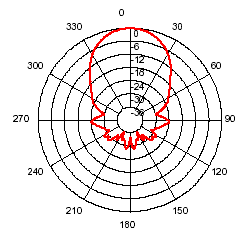
\includegraphics[scale=0.5]{us-beam.png}
	\caption{Haz ultras\'onico del sensor de distancia por ultrasonido SRF05.}
	\label{HFultrasonido}
\end{figure}

\subsubsection{Tel\'emetros infrarrojos}
\label{HStelemetros}

Los tel\'emetros por infrarrojo que elegimos son el modelo \emph{GP2D120} de Sharp \footnote{http://sharp-world.com/products/device}.

El principio de funcionamiento de este tipo de sensores es mediante un haz de luz infrarroja que es emitido hacia el objetivo, el cual
es reflejado y captado a traves de un lente por un sensor de posici\'on relativa en el interior del sensor. En base a esta medici\'on
se calcula la distancia entre el sensor y el objeto reflectivo que se encuentra frente a \'el. La salida es anal\'ogica para este
modelo espec\'ifico. En la tabla \ref{HTtel} detallamos los valores caracter\'isticos del modelo.

\begin{table}
	\begin{center}
		\begin{tabular}{|l|c|c|}
			\hline
			Caracter\'istica & Unidad & Valor\\
			\hline
			Rango m\'aximo & $cm$ & 30 \\
			Rango m\'inimo & $cm$ & 4 \\
			Tensi\'on para la m\'axima distancia & $V$ & 1.95 \\
			Tensi\'on para la m\'inima distancia & $V$ & 2.55 \\
			Tensi\'on de alimentaci\'on & $V$ & 5 \\
			Consumo m\'aximo & $mA$ & 50 \\
			\hline
		\end{tabular}
	\end{center}
	\caption{Caracter\'isticas del sensor de distancia por ultrasonido SRF05.}
	\label{HTtel}
\end{table}

En la figura \ref{HFteldistancia} mostramos la tabla de conversi\'on entre voltaje de salida y distancia al objeto, y en la figura 
\ref{HFtelapertura} mostramos el \'angulo de apertura de la zona de detecci\'on seg\'un la distancia al objetivo.

\begin{figure}[ht]
	\centering
	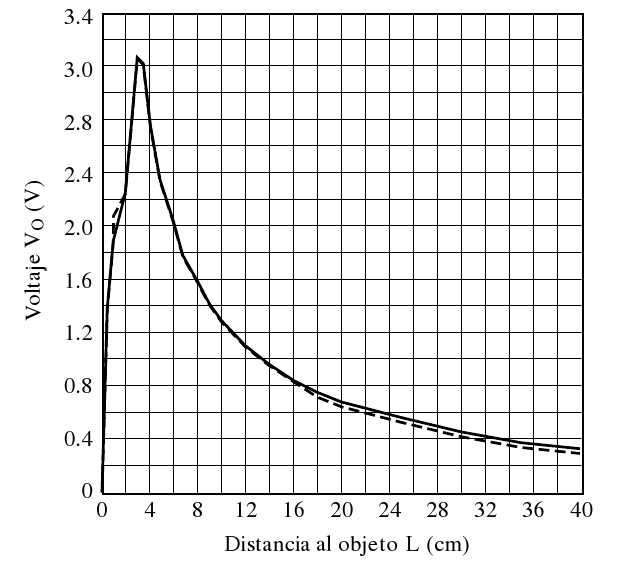
\includegraphics[scale=0.35]{tel-VxL.png}
	\caption{Haz ultras\'onico del sensor de distancia por ultrasonido SRF05.}
	\label{HFteldistancia}
\end{figure}


\begin{figure}[ht]
	\centering
	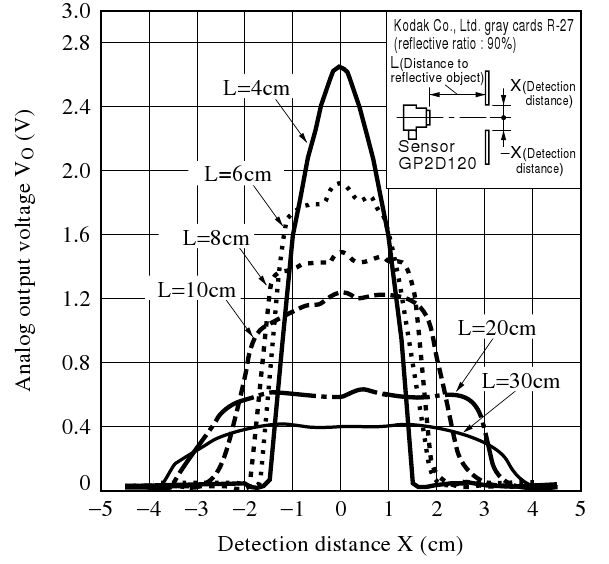
\includegraphics[scale=0.35]{tel-VxX.png}
	\caption{Haz ultras\'onico del sensor de distancia por ultrasonido SRF05.}
	\label{HFtelapertura}
\end{figure}

\subsubsection{Sensores reflectivos de piso}
\label{Hpiso}

Los sensores que elegimos para sensar la l\'inea reflectiva en el piso son el modelo \emph{CNY70} de la marca Vishay Semiconductor
\footnote{http://www.vishay.com/}.

Son sensores opticos reflectivos que captan el nivel de luz emitida por el mismo sensore y reflejada sobre la superf\'icie a sensar
como se muestra en la figura \ref{HFpiso}. En la figura \ref{HFpisoID} 

El rango efectivo de sensado ronda los $3 mm$ de distancia, aunque con un incremento en la corriente que circula por el emisor de luz
se puede llegar a una distancia mayor que permita un uso m\'as acorde al proyecto.

\begin{figure}[ht]
	\centering
	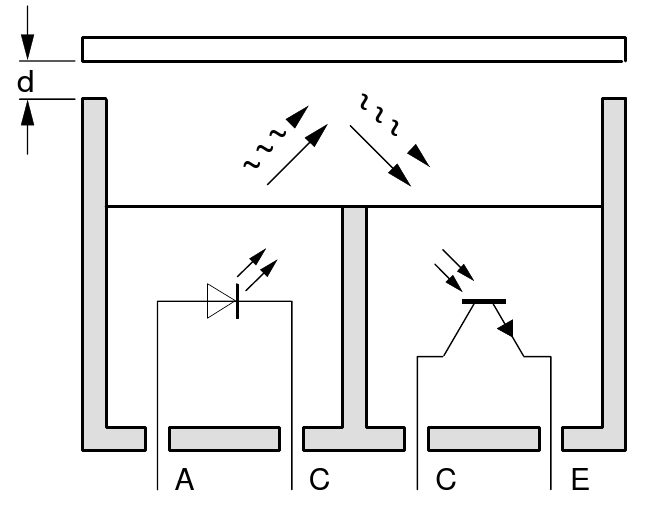
\includegraphics[scale=0.15]{piso.png}
	\caption{Principio de funcionamiento del sensor reflectivo CNY70.}
	\label{HFpiso}
\end{figure}


\begin{figure}[ht]
	\centering
	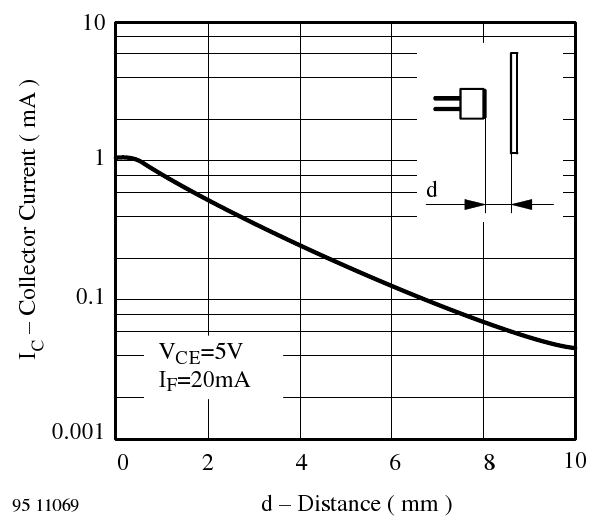
\includegraphics[scale=0.35]{piso-IxD.png}
	\caption{Corriente que circula por el colector seg\'un la distancia al objetivo en el sensor CNY70.}
	\label{HFpisoID}
\end{figure}

\subsubsection{Sensado de nivel de bateria}
\label{HSnivelBateria}

El sensado del nivel de tensi\'on en la bater\'ia lo hacemos mediante un divisor de tensi\'on entre los polos de la bater\'ia misma
y sensados de igual forma que los otros sensores. En la secci\'on \ref{HAPsensores} explicamos mas en detalle la conexi\'on.
En la figura \ref{HFbateria} mostramos el diagrama del divisor de tensi\'on.

\begin{figure}[ht]
	\centering
	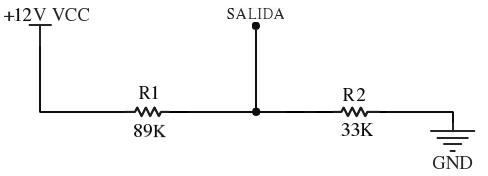
\includegraphics[scale=0.35]{bateria.png}
	\caption{Divisor de tensi\'on para el sensado de la bater\'ia.}
	\label{HFbateria}
\end{figure}

En la tabla \ref{HTdivT} mostramos las posibles tensiones en la bater\'ia y la tensi\'on de salida en el divisor. Tambi\'en incluimos el
valor aproximado para un conversor anal\'ogico digital con tensi\'on de referencia a $5V$ que leer\'a la salida del divisor.

\begin{table}
	\begin{center}
		\begin{tabular}{|c|c|c|c|}
			\hline
			Bater\'ia ($V$) & Salida ($V$) & Valor en el ADC ($5V$) \\
			\hline
			16 & 4.327 & 886 \\
			15 & 4.057 & 831 \\
			14 & 3.786 & 776 \\
			13 & 3.516 & 720 \\
			12 & 3.245 & 665 \\
			11 & 2.975 & 609 \\
			10 & 2.704 & 554 \\
			 9 & 2.434 & 499 \\
			 8 & 2.163 & 443 \\
			 7 & 1.893 & 388 \\
			 6 & 1.623 & 332 \\
			 5 & 1.352 & 277 \\
			\hline
		\end{tabular}
	\end{center}
	\caption{Tensi\'on de la bater\'ia y la tensi\'on de salida en el divisor.}
	\label{HTdivT}
\end{table}

\subsubsection{Encoders y consumo de los motores}
\label{HSencodersConsumo}

Encoders y sensado del consumo de los motores

\subsection{Comunicaci\'on entre m\'odulos}
\label{Hcomm}

comunicacion - comunicacion entre placas y con la pc, protocolo

\subsubsection{Conectividad entre los m\'odulos de control}
\label{HCconectividad}

comuncacion entre las placas, daisy chain, diagrama de conexionado.
comm con la pc, serial.
velocidad de transmision, control de flujo, deteccion de errores por soft en el protocolo no por hard.

\subsubsection{Protocolo de comunicaci\'on}
\label{HCprotocolo}

protocolo, paquetes. Apendice?
retransmision, control de errores.

\subsection{El microcontrolador}
\label{Hmicro}

microcontrolador elegido, familia, caracteristicas, memoria, modulos disponibles, IOs, interrupciones

\subsubsection{RS-232}
\label{HMrs232}

rs232 en el micro. donde se usa

\subsubsection{Timers}
\label{HMtimers}

timers en el micro. donde se usan

\subsubsection{PWM}
\label{HMpwm}

PWM en el micro. donde se usa

\subsubsection{ADC}
\label{HMadc}

ADC en el micro. donde se usa

\subsubsection{Programador}
\label{HMprogramador}

programador, pines de programacion, switch, IDE, lenguaje de programacion.

\subsection{Armado f\'isico del prototipo}
\label{Harmado}

\emph{armado fisico -> placas, ruedas, chasis, bateria, netbook}

\subsubsection{Placa gen\'erica}
\label{HAPgenerica}

placa base - principio de funcionamiento, diseño y circuito a un apendice?
comunicacion, configuracion, modulo para la comunicacion, pines, conectores, switch

\subsubsection{Placa controladora de motor de continua}
\label{HAPmotorDC}

controladora de motorDC.
principio de funcionamiento.
configuracion x hardware, valores maximos y minimos que soporta.
diseño y circuito a un apendice?

\subsubsection{Placa controladora de sensores}
\label{HAPsensores}

controladora de sensores.
principio de funcionamiento.
diferenciacion entre los tipos de sensores que pueden conectarse, a donde van.
rangos de voltaje soportados, valores y configuracion x hardware.
diseño y circuito a un apendice?

\subsubsection{Placa controladora de servo motores}
\label{HAPservos}

controladora de servos.
principio de funcionamiento.
configuracion x hardware, valores maximos y minimos que soporta.
diseño y circuito a un apendice?

\subsubsection{Controlador principal}
\label{HAPprincipal}

eleccion de la netbook.
especificaciones, caracteristicas, peso, bateria.


\subsubsection{Accesorios de construcci\'on}
\label{HAaccesorios}

eleccion de la bateria, ruedas.
especificaciones.

\subsubsection{Construcci\'on del prototipo}
\label{HACprototipo}

eleccion de los materiales de construccion y armado final.
planos.

\subsection{Conclusi\'on}
\label{Hconclusion}

\emph{posibles extensiones}
